%File: formatting-instruction.tex
\documentclass[letterpaper]{article}
\usepackage{url,graphicx,xcolor}
\usepackage{times}
\usepackage{helvet}
\usepackage{courier}
\usepackage{hyperref}
%\usepackage[guidelines]{faikrmod3}
\usepackage[]{faikrmod3} % without guidelines
\frenchspacing
\setlength{\pdfpagewidth}{8.5in}
\setlength{\pdfpageheight}{11in}



% THE \pdfinfo /Title AND /Author ARE NOT NECESSARY, THEY ARE METADATA FOR THE FINAL PDF FILE
\pdfinfo{
/Title (Heart Disease Risk Assessment using Bayesian Networks)
/Author (Matteo Fasulo, Luca Tedeschini, Antonio Gravina, Luca Babboni)}
\setcounter{secnumdepth}{0}  
 \begin{document}
% The file aaai.sty is the style file for AAAI Press 
% proceedings, working notes, and technical reports.
%
\title{Heart Disease Risk Assessment using Bayesian Networks}
\author{Matteo Fasulo, Luca Tedeschini, Antonio Gravina, Luca Babboni\\
Master's Degree in Artificial Intelligence, University of Bologna\\
\{ matteo.fasulo, luca.tedeschini3, luca.babboni2, antonio.gravina \}@studio.unibo.it
}

\maketitle


\attention{DO NOT MODIFY THIS TEMPLATE - EXCEPT, OF COURSE FOR TITLE AND AUTHORS. REMOVE THE \texttt{guidelines} OPTION FROM  \texttt{$\backslash$usepackage[guidelines]\{faikrmod3\}} IN THE \LaTeX\ SOURCE IN THE FINAL VERSION.}

\begin{abstract}
\begin{quote}

\explanation{
This mini-project aims to ... \\
We use ... \\
We found that ...
}

Cardiovascular diseases (CVDs), the leading cause of death globally, claimed an estimated 17.9 million lives in 2019, accounting for 32\% of all global deaths. Of these, 85\% were due to heart attack and stroke, with over three quarters occurring in low- and middle-income countries. Furthermore, CVDs were responsible for 38\% of the 17 million premature deaths (under the age of 70) due to noncommunicable diseases in 2019. Most CVDs can be prevented by addressing behavioural risk factors such as tobacco use, unhealthy diet, obesity, physical inactivity, and harmful use of alcohol \cite{WHO2024}. \\
In this context, our study employs Bayesian networks (BNs) for early detection of CVDs, which is crucial for effective management through counselling and medicines. Inspired by this paper \cite{ORDOVAS2023107405}, we apply their approach to a new dataset combined from different data sources. Our aim is to validate the effectiveness of BNs in predicting CVD risk and to analyze the interactions between various risk factors. This work contributes to the early detection and management of CVDs, potentially reducing its health and economic impact.

\end{quote}
\end{abstract}


\section{Introduction}
\subsection{Domain}
\explanation{
Introduce your work: what you are modeling, if you are drawing inspiration from an existing model, study, paper, textbook example, challenge, \dots.\\
%
Briefly provide whatever background information on the domain you think is necessary for the reader to understand the model and your design choices.
}

In our study, we are modeling the risk of cardiovascular diseases (CVDs), a leading cause of death globally \cite{WHO2024}. Our model aims to predict the likelihood of CVDs based on a range of risk factors, such as age, sex, chest pain type, resting blood pressure, cholesterol levels, and more. \\
Our work draws inspiration from a paper \cite{ORDOVAS2023107405}, where the authors developed a Bayesian network (BN) to predict CVD risk. Bayesian networks are a powerful tool for handling complex data and analyzing the interactions between various risk factors. We aim to replicate their approach using a different dataset, thereby validating the effectiveness of BNs in predicting CVD risk.\\
The domain of our study is healthcare, specifically cardiovascular health. 
Since the 1930s, research has identified diverse CVD risk factors \cite{MAHMOOD2014999}. Notably, CVDs encompass a range of conditions, including heart disease and stroke, and are often associated with modifiable risk factors such as hypertension, diabetes, and hyperlipidaemia. Early detection and management of these risk factors are crucial in reducing the incidence and impact of CVDs. \\
Our choice of using a Bayesian network as our model is motivated by its ability to handle complex, real-world data and its success in healthcare applications \cite{nielsen2009bayesian}. Furthermore, BNs allow us to analyze how various risk factors interact, providing valuable insights into the mechanisms of CVDs.

\attention{HERE AND EVERYWHERE ELSE: ALWAYS KEEP IN MIND THAT, CRUCIALLY, WHATEVER TEXT/CODE/FIGURES/IDEAS/... YOU TAKE FROM ELSEWHERE MUST BE CLEARLY IDENTIFIED AND PROPERLY REFERENCED IN THE REPORT.}

\subsection{Aim}
\explanation{
Explain the purpose of your project: what do you intend to observe/try/experience/\dots? \\
\begin{itemize}
    \item 
Example: the purpose of this project is to implement part of the Bayesian network described in \cite{10.1371/journal.pone.0220065} and experiment with concepts seen in class \\
%
\item Another example: our aim was to experiment the effect of discretization of continuous variables \\
%
\item Yet another example: we are interested in comparing the run-time and error of approximate inference under different conditions
%
\item One final example: we studied \textit{value of information}: something mentioned in class but not covered in this module, which sparked our interest.
\end{itemize}
}\\
The purpose of our project is to develop a Bayesian Network (BN) classifier that predicts the presence or absence of heart disease. Our primary goal is to maximize the F-beta score, which is a measure of a test's accuracy. It considers both precision (the number of true positive results divided by the number of all positive results) and recall (the number of true positive results divided by the number of results that should have been identified as positive). The beta parameter in the F-beta score determines the weight of recall in the combined score. \\
In addition to this, we are also interested in the process of discretizing continuous variables such as cholesterol levels and maximum heart rate. We will be dividing these variables into bins based on standard values referenced in the literature. This method can help handle continuous variables more effectively in our BN model.\\
Through this project, we aim to observe the performance of the BN model in predicting heart disease, experiment with different methods of discretization and parameter tuning, and gain experience in working with real-world healthcare data and Bayesian networks. Ultimately, we hope to create a model that can accurately predict the risk of heart disease, contributing to early detection and prevention efforts.

\subsection{Method}
\explanation{
Describe the methodology you followed
\begin{itemize}
    \item 
Example: we used pgmpy library methods\footnote{This is just an example: indeed, it is NOT necessary to use pgmpy; the coding language doesn't have to be python either. Feel free to use whatever software framework suits your needs.} to implement our network and run queries. To understand if differences in models, queries, parameters or number of samples induced differences in accuracy, we varied evidence nodes, conditional probability distributions, inference method, ...
\end{itemize}
}

In our project, we followed a systematic methodology to construct a Bayesian Network (BN) for predicting heart disease. We used the `pgmpy` library, a Python library for probabilistic graphical models, to construct our BN. Our data was split into a training set and a testing set in an 80-20 ratio. This allowed us to train our model on a majority of the data and then test its performance on unseen data. \\
To understand if differences in the model would produce better F-beta scores, we varied the structure of our BN using a structure learning approach. This approach was augmented with domain knowledge that we found in the literature, which helped guide the structure learning process. \\
In addition to varying the structure, we also varied the scoring method used by the structure learning algorithm. This was done to find the optimal (unparametrized) network structure. By varying both the structure and the scoring method, we aimed to explore different configurations of our model and identify the one that maximizes the F-beta score.

\subsection{Results}

\explanation{
In a few lines: what are the most noteworthy results you have observed or things you have learned/understood from this project? (only the highlights: there will be a dedicated paragraph for presenting results in the Analysis section)
}

From this project, we observed that the F-beta score, a crucial metric for our model's performance, is highly influenced by the structure of the Bayesian Network (BN). \\
We found that the unconstrained model, while yielding a slightly higher F-beta score, included meaningless edges. This is likely due to the optimization of a scoring function of the structure given the data, without any knowledge of the meaning of the features. \\
On the other hand, the constrained model, which was driven by domain knowledge, was still able to explain most of the data correlations while also accounting for more meaningful edges.
\section{Model}

\explanation{
Insert a picture of your Bayesian network(s) (Figure~\ref{fig:network})
%
\begin{figure}
    \centering
    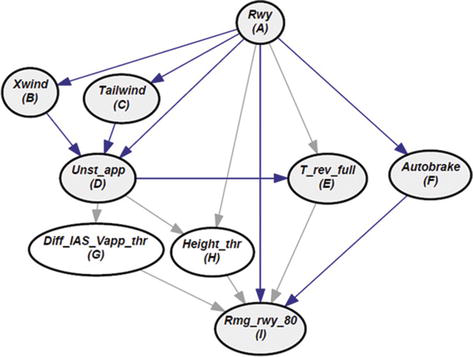
\includegraphics[scale=1.0]{F2.png}
    \caption{Bayesian network. Image taken from \url{https://www.intechopen.com/chapters/62844}}
    \label{fig:network}
\end{figure}
}

\begin{figure}
    \centering
    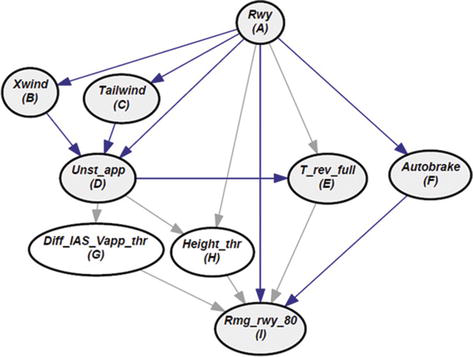
\includegraphics[scale=1.0]{F2.png}
    \caption{Bayesian network. Image taken from \url{https://www.intechopen.com/chapters/62844}}
    \label{fig:network}
\end{figure}

\explanation{
Explain the following aspects of your model (if there is too much to say and not enough space, put in your notebook whatever does not fit here):
\begin{itemize}
    \item nodes: if not self-explanatory, explain each random variable's meaning/intuition and type/range
    \item conditional distributions (for example, the CPTs, some or all of them)
    \item the procedure you followed to build your model (structure and conditional distributions): from reference paper? by analyzing the domain? learned from data? just assigned probability distributions arbitrarily? followed a particular methodology for building the network? ...
\end{itemize}  
In general, only write whatever is relevant and necessary to understand the rest of the report. Do not explain concepts seen in class or explained in textbooks. Do not describe models taken from textbook/literature/tutorials/libraries, like (for example) the Asia network. Instead, if you are using a model as-is: just insert a reference or URL\footnote{\url{https://www.bnlearn.com/bnrepository/}.}
}

In our model each node is a random variable with a specific meaning and range. For instance, “Age” represents the age of the patient in years, “Sex” indicates the patient’s gender, and “ChestPainType” denotes the type of chest pain experienced by the patient. Other nodes include “RestingBP” (resting blood pressure), “Cholesterol” (serum cholesterol level), “FastingBS” (fasting blood sugar), “RestingECG” (resting electrocardiogram results), “MaxHR” (maximum heart rate achieved), “ExerciseAngina” (exercise-induced angina), “Oldpeak” (oldpeak = ST), “ST\_Slope” (the slope of the peak exercise ST segment), and “HeartDisease” (the presence or absence of heart disease).\\
In addition to the construction of the BN, we also performed discretization on the continuous variables in our dataset using standard values found in literature about the features. A more in-depth explanation of the ranges and labels of the discretized variables is available in the notebook.\\
The conditional distributions of these nodes, such as the Conditional Probability Tables (CPTs), were learned from the data.\\
We followed a hybrid approach to build our BN. Initially, we used a local search algorithm, specifically hill climbing, to find the structure that best explains the correlations in our data. This was done not with the fitted model but just with the structure.\\
After obtaining a solution from the hill climbing algorithm, we identified some edges that did not make sense in the context of our domain. We added these edges to a blacklist, effectively constraining the network structure.\\
We then ran the hill climbing algorithm again, but this time with these constraints. This allowed us to find a structure that was both statistically sound and made sense in the context of heart disease prediction.\\
Finally, we made some modifications to the edges based on literature references to ensure the causal meaning of the edges in the BN. This process allowed us to speed up the computation by first finding a good initial structure and then refining it based on domain knowledge and constraints.\\
Through this project, we intend to observe the effectiveness of BNs in predicting heart disease and gain insights into the interactions between various risk factors. We also aim to experiment with the effect of different network structures and constraints on the prediction accuracy.

\section{Analysis}

\subsection{Experimental setup}
\explanation{
Briefly describe the probability queries or other experiments that you have carried out. Describe how you plan to evaluate the results (for example: are there results that you would expect?)
}
To evaluate the results, we used the F-beta score with beta set to 2, which makes recall twice as important as precision. This is particularly relevant in medical diagnosis where it is crucial to minimize the rate of false negatives \cite{9418099}. In other words, it is more important to correctly identify all actual positive cases (high recall) even at the expense of including some false positives (lower precision). This is because a false negative, or failing to identify a true case of heart disease, could have serious, potentially life-threatening repercussions. Therefore, a model with a higher recall is more desirable in this context.\\
This approach aligns with the general consensus in the field that in high-risk disease detection cases like heart disease, recall is a more important evaluation metric than precision. We expect that a model with a higher recall will be more effective in predicting heart disease, thereby contributing to early detection and prevention efforts while still maintaining a good precision score.

\subsection{Results}
\explanation{
What did you observe? \\
%
All according to expectations? \\
%
Anything surprising or worthwhile mentioning?
}


\section{Conclusion}
\explanation{
Just one paragraph: what you have learned, anything interesting that came up, what are the limitations of your model/experiments/study/...
}


\section{Links to external resources}
\explanation{
Optionally, insert here:
\begin{itemize}
    \item a link to your GitHub or any other public repo where one can find your code (only if you did not submit your code on Virtuale) 
    \item a link to your dataset (only if you have used a dataset, for example, for learning network parameters or structure)
\end{itemize}
Leave this section empty if you have all your resources in Virtuale. \textbf{Do not insert code/outputs in this report}.
}
The notebook containing the project is available on \href{https://github.com/MatteoFasulo/BayesianClassifier}{GitHub}. Refer \cite{dataset} for the dataset.
\bigskip

\bibliographystyle{aaai}
\bibliography{faikrmod3.bib}


\attention{NOTICE: THIS REPORT'S LENGTH MUST NOT EXCEED \textbf{TWO PAGES} PLUS REFERENCES. THIS MAY MEAN THAT YOU WILL HAVE TO LEAVE OUT OF THE REPORT PART OF THE WORK YOU HAVE DONE OR OBSERVATIONS YOU HAVE. THIS IS NORMAL: THE REPORT SHOULD EMPHASIZE WHAT IS MOST SIGNIFICANT, NOTEWORTHY, AND REFER TO THE NOTEBOOK FOR ANYTHING ELSE. FOR ANY OTHER ASPECT OF YOUR WORK THAT YOU WOULD LIKE TO EMPHASIZE BUT CANNOT EXPLAIN HERE FOR LACK OF SPACE, FEEL FREE TO ADD COMMENTS IN THE NOTEBOOK.}


\end{document}